\documentclass{article}
\usepackage{xspace}
\usepackage[utf8]{inputenc}
\usepackage[T1]{fontenc}
\usepackage[english]{babel}
\usepackage{amsmath}
\usepackage{amsthm}
\usepackage{graphicx}
\usepackage{url}
\usepackage{amssymb}
\usepackage{algorithme}
\usepackage{mathrsfs}
\usepackage{amsfonts}
\usepackage{multicol}
\usepackage{stmaryrd}
\usepackage{tikz, pgf}
\usetikzlibrary{arrows,intersections}
\usepackage{libertine}
\usepackage[a4paper,left=2cm,right=2cm,top=2cm,bottom=2cm]{geometry}
\usepackage{dsfont}


\usepackage[linktocpage]{hyperref}

\setlength{\hoffset}{-18pt}         
\setlength{\oddsidemargin}{15pt} % Marge gauche sur pages impaires
\setlength{\evensidemargin}{15pt} % Marge gauche sur pages paires
\setlength{\marginparwidth}{0pt} % Largeur de note dans la marge
\setlength{\textwidth}{481pt} % Largeur de la zone de texte 
\setlength{\marginparsep}{7pt} % Séparation de la marge
\setlength{\topmargin}{0pt} % Pas de marge en haut
\setlength{\headheight}{13pt} % Haut de page
\setlength{\headsep}{10pt} % Entre le haut de page et le texte
\setlength{\footskip}{50pt} % Bas de page + séparation
\setlength{\textheight}{600pt} % Hauteur de la zone de texte 

%\setlength{\hoffset}{-18pt}         
%\setlength{\oddsidemargin}{15pt} % Marge gauche sur pages impaires
%\setlength{\evensidemargin}{15pt} % Marge gauche sur pages paires
%\setlength{\marginparwidth}{0pt} % Largeur de note dans la marge
%\setlength{\textwidth}{481pt} % Largeur de la zone de texte 
%\setlength{\marginparsep}{7pt} % Séparation de la marge
%\setlength{\topmargin}{0pt} % Pas de marge en haut
%\setlength{\headheight}{8pt} % Haut de page
%\setlength{\headsep}{0pt} % Entre le haut de page et le texte
%\setlength{\footskip}{15pt} % Bas de page + séparation
%\setlength{\textheight}{700pt} % Hauteur de la zone de texte 

%\newcommand{\ket}[1]{\ensuremath{|#1\rangle}\xspace}
%\newcommand{\bra}[1]{\ensuremath{\langle #1|}\xspace}

\newtheorem{thm}{Theorem}[section]
\newtheorem{prop}[thm]{Proposition}
\newtheorem{lem}[thm]{Lemma}
\newtheorem{cor}[thm]{Corollary}
\newtheorem{defi}[thm]{Definition}
\newtheorem{ex}[thm]{Example}

\newcommand{\Thm}[3]{\begin{thm}[#1]\label{#2}#3\end{thm}}
\newcommand{\Ex}[3]{\begin{ex}[#1]\label{#2}#3\end{ex}}
\newcommand{\Def}[3]{\begin{defi}[#1]\label{#2}#3\end{defi}}
\newcommand{\Lem}[3]{\begin{lem}[#1]\label{#2}#3\end{lem}}
\newcommand{\Cor}[3]{\begin{cor}[#1]\label{#2}#3\end{cor}}
\newcommand{\Prop}[3]{\begin{prop}[#1]\label{#2}#3\end{prop}}

\newcommand{\Rem}{\underline{Remark:} }
\newcommand{\Idea}{\underline{Idea:} }
\newcommand{\Question}{\underline{Question:} }

\newcommand{\hsp}{\hspace{20pt}}
\newcommand{\HRule}{\rule{\linewidth}{0.5mm}}
\newcommand{\R}{\mathbb{R}}
\newcommand{\N}{\mathbb{N}}
\newcommand{\K}{\mathbb{K}}
\newcommand{\Q}{\mathbb{Q}}
\newcommand{\C}{\mathcal{C}}
\newcommand{\A}{\mathcal{A}}
\newcommand{\B}{\mathcal{B}}
\newcommand{\X}{\mathcal{X}}
\newcommand{\brakets}[1]{\langle#1\rangle}
\newcommand{\half}{\frac{1}{2}}
\newcommand{\bit}{\{0,1\}}

\newcommand{\ind}[1]{\mathds{1}_{#1}}
\renewcommand{\epsilon}{\varepsilon}

\title{Cryptography}
\author{Benoit Libert et Damien Stehlé	}
\date{Spring 2017}



\begin{document}

\maketitle

\tableofcontents

\newpage

\section{Introduction}
Cryptography is the science of information security, not just encryption. In a sense it is not just Information Theory.

The most classical form of encryption must satisfy:
\begin{itemize}
\item A talks to $B$ over a public channel
\item We don't want any eavesdropper (oreille indiscrète) C to understand the communication.
\end{itemize}

\Ex{}{}{Take a client and a server such that each of them have a browser with 2 stages:
\begin{itemize}
\item 1: Handshake. They create a common session key, $K$
\item 2: Using $K$, they can encrypt and decrypt the communication.
\end{itemize}

We will see the first step later, and in the following we will shortly deal with the second.
}

We have to deal with:
\begin{itemize}
\item Secret key cryptography: $A$ and $B$ use the same secret key $K$ to communicate
\item Cryptography is not just an encryption:
\begin{itemize}
\item How $A$ can be sure he is really talking to $B$ (use of digital signatures)
\item How can they know the that the communication has not been modified ? (Question of integrity)
\item What if I don't want to reveal my identity ? (Anonymous communication)
\end{itemize} 
\item More complex primitives and properties:
\begin{itemize}
\item Digital cash: should be anonymous, infeasible to fake or duplicate
\item E-voting: $n$ voter choose candidates, majority wins but votes should be anonymous, it must impossible to vote twice, votes must not be verified.
\end{itemize}
\end{itemize}

Cryptography is a science on its own. It has its own methodology. Basically, we can sum it up in this few steps:
\begin{itemize}
\item One defines what the protocol has to do
\item One defines the attacker's goal and power. The aim is to give a security model.
\item One describes a protocol realisation
\item One «proves» that, if an «efficient» attacker exists, then some hard problem can be solved (e.g. factoring, computing discrete logarithms).
\end{itemize}

Cryptography often plays with some hard problems. It is a kind of face of complexity theory. It always suppose that protocols' specifications and description are public, the adversary knows how the protocol works, only the key remains private (Kerckhoff's principle).

However cryptography has its limitations:
\begin{itemize}
\item it relies on algorithmic assumptions and does not ensure unconditional security.
\item does not protect against engineering bugs (FREAK attack (2015), attack intercepts https connections and forces client/server to use weak encryption, or LOGJAM attack (2015), client/server forced to use too short keys)
\item some attacks are out-of-model exists: side-channel information (e.g. power consumption may leak the key)
\item backdoors may be correctly introduced in cryptographic implementations
\item security threats may be unrelated to cryptography
\end{itemize}

\section{One-time pad and perfect security}
\Def{Encrytion Scheme}{def:encrysch}{An encryption scheme $(Keygen, Enc, Dec)$ operates over finite sets $(K,P,C)$ with:
\begin{itemize}
\item $Keygen$ chooses $k$ uniformly in $K$
\item $Enc : K\times P \rightarrow C$
\item $Dec : K\times C \rightarrow P$
\end{itemize}
such that $\forall m\in P, k\in K, Dec(k,Enc(k,m))=m$ and such there are PPT (probabilistic polynomial time) algorithms that compute each of those previous functions.
\begin{itemize}
\item $m$ and $k$ are independent random variables
\item $Enc$ may be probabilistic but $Dec$ is usually deterministic
\item We assume (in the following) that elements of $K,P,C$ have non-zero probabilities.
\end{itemize}}

\Def{Perfect security (Shannon, 1949)}{def:perfSec}{For any message distribution $\mathcal{M}$ over $P$, \[\forall \overline{m}\in P, \Pr_{m\hookrightarrow\mathcal{M}, k\hookrightarrow U(K)}(m=\overline{m}|Enc(k,m))=\Pr(m=\overline{m})\]}

\underline{Remark:} The intuition is that giving $E(k,m)$ does not leaks any information about $m$. Formally, $m$ and $Enc(k,m)$ are independent.

\Lem{Shannon}{}{Perfect security implies that $|K|\geq|P|$}
\begin{proof}
By contradiction assume $|K|<|P|$. Then define $P(\bar{c})=\{m\in P|\exists k\in K, m=Dec(k,\bar{c})\}$. Then $|P(\bar{c})|\leq|K|$ since $\forall m\in P(\bar{c}),\exists k\in K, m=Dec(k,\bar{c})$.

Then by our assumption $P-P(\bar{c})\neq\emptyset$. Let $\bar{m}$ be in this set. Then $\Pr(m=\bar{m}|\bar{c}=Enc(k,m))=0\neq\Pr(m=\bar{m})$. That is a contradiction with perfect security (ck previous remark).
\end{proof}

\Def{One-time Pad (OTP), Vernam's cipher (patented in 1917)}{def:OTP}{We take $K=\{0,1\}^l=P=C$. $Enc(k,m) = m\oplus k$ and $Dec(k,c)=c\oplus k$}

\Thm{}{thm:OTPPerfect}{Vernam's cipher is perfectly secret}
\begin{proof}
Let $\bar{m}\in P, \bar{c}\in C$ arbitrary. If we have $\Pr(c=\bar{c}|m=\bar{m})=\Pr(c=\bar{c}))=\Pr(c=\bar{c})$ then by multiplying by $\frac{\Pr(m=\bar{m})}{\Pr(c=\bar{c})}$ we get the result. Then let's compute it:
\[\begin{array}{r c l}
\Pr(c=\bar{c}|m=\bar{m}) & = & \Pr(m\oplus k=\bar{c}|m=\bar{m})\\
&=&\Pr(\bar{m}\oplus k \bar{c})\\
&=&\frac{1}{2^l}
\end{array}\]
\[\begin{array}{r c l}
\Pr(c=\bar{c}) & = & \sum_{\bar{m}}\Pr(\bar{c}=\bar{c}|m=\bar{m})\Pr(\bar{m}=m)\\
&=&\frac{1}{2^l}\sum_{\bar{m}}\Pr(\bar{m}=m)\\
&=&\frac{1}{2^l}
\end{array}\]
\end{proof}

The major problems with that are:
\begin{itemize}
\item key is as long as the message
\item we cannot encrypt twice with the same key ($Enc=Dec$)
\item Assumes an unbounded adversary (too powerful)
\end{itemize}

\section{Pseudo-random generators (PRG) and stream ciphers}
\subsection{One-time pad and pseudo-randomness}
\underline{Idea:} use the OTP with pseudo-random bits rather than truly random ones.

\begin{itemize}
\item We want to use a PRG $G:\{0,1\}^s\rightarrow\{0,1\}^n$ with $n\gg s$
\item Input $k\in\{0,1\}^s$, called \underline{seed} and contains all the randomness
\item $G$ is computable in deterministic polynomial time
\item Tempting idea for encryption: $Enc(k,m) = m\oplus G(k)$ and $Dec(c,k) = c\oplus k$ ($m\in\{0,1\}^n$ is longer than $s$).
\end{itemize}
\underline{Question:} Perfect secrecy is impossible. Can we get computational security ?

\Def{Negligible function}{def:negligFunc}{$f:\N\rightarrow\R$ is negligible if $\forall c>0,\exists n_0\in\N, \forall n>n_0,|f(n)|<n^{-c}$}

\Ex{}{}{$2^{-n}$, $n^{-\log n}$... are negligible functions of $n$.}

\Prop{}{}{For any negligible function $\epsilon$, for any polynomial $P$, the product $P(n)\epsilon(n)$ is still negligible}

\Def{Predictable PRG}{def:predPRG}{
A PRG is \underline{predictable} if there exists a PPT (Probabilistic Polynomial Time) algorithm $A$ and an index $i\in\llbracket1,m\rrbracket$ such that:
\[\Pr_{k\hookrightarrow U(\{0,1\}^s), \text{$A$'s internal randomness}}(A(G(k)[1...i])=G(k)[i+1])>\frac{1}{2}+\epsilon(s)\]
for some non-negligible function of $s$, $\epsilon>0$.}
\underline{Remark:} It restricts the adversary's power (otherwise $A$ could use all possible $k$) and the probability is taken over the uniform choice of $k$ and the internal randomness of $A$.

\underline{Remark: } A PRG is unpredictable if for all PPT algorithm and index, $\epsilon$ is negligible.

\underline{Question: } How to compute $p:=\Pr_{k\hookrightarrow U(\{0,1\}^s), \text{$A$'s internal randomness}}(A(G(k)[1...i])=G(k)[i+1])$ ? One way to do so is to proceed as the following algorithm:\\


\begin{algorithme}
$x::=0$\\
\ForFromTo{i}{1}{N}{choose $k$ uniformly at random\\
If $A(G(k)[1...i])=G(k)[i+1]$ increment $x$}
\Return{$x/N\approx p$}
\end{algorithme}

Using Hoeffding bound we get $\Pr(|x-pN|\geq t)\leq 2\exp(-2t^2/N)$, then $\Pr(|x-pN|\geq t'\sqrt{N})\leq 2\exp(-2t'^2)$ for any $t'$. Then we get $p$ with approximation $1\pm\frac{10}{\sqrt{N}}$ with $t'=10$.


\Def{Distinguishability}{def:disting}{Let $D_1$ and $D_2$ be two distributions. They are distinguishable if there is a PPT algorithm $\mathcal{A}:\{0,1\}^n\rightarrow\{0,1\}$ with support $\{0,1\}^n$ such that $Adv_\mathcal{A}(D_1,D_2) := |\Pr_{x\hookrightarrow D_1}(\mathcal{A}(x)=1)-\Pr_{x\hookrightarrow D_2}(\mathcal{A}(x)=1)|$ is non-negligible. Then $\mathcal{A}$ is a distinguisher for $D_1$ and $D_2$.}

$G(\{0,1\}^s)$ is a tiny subset of $\{0,1\}^n$ but we want it to looks uniform. We want it is indistinguishable from the uniform distribution.

\Def{Indistinguishability}{def:indisting}{$D_1$ and $D_2$ are indistinguishable if for any PPT $\mathcal{A}:\{0,1\}^n\rightarrow\{0,1\}$ $Adv_\mathcal{A}(D_1,D_2)$ is negligible.}

\Def{Indistinguishability from uniform}{def:unifPRG}{A PRG $G$ is indistinguishable from uniform if $D_1:=\{G(k)|k\hookrightarrow U(\{0,1\}^s)\}$ and $D_2:=\{x|x\hookrightarrow U(\{0,1\}^n)\}$ are indistinguishable} 

\Def{unpredicatable PRG}{def:unpredPRG}{A PRG $G$ is unpredictable if for every PPT algorithm $\A$ and every $i\in\{1,...,n\}$,
\[|\Pr_{k\hookrightarrow U(\{0,1\}^s)}(\A(G(k)[1...i])=G(k)[i+1])-\frac{1}{2}|\leq negl(s)\]
for some $negl:\N\rightarrow\N$.
}

\Rem Statistical distinguishers always exist. A random $x\hookrightarrow U(\{0,1\}^n)$ belongs to $G(\{0,1\}^s)$ with proba $\frac{1}{2^{n-s}}$. Distinguisher can try all possible $k\in\{0,1\}^s$ (we just hope it is to costly).

\Thm{}{thm:indisUnpredEquiv}{Definition \ref{def:unpredPRG} and \ref{def:unifPRG} are equivalent.}

\begin{proof}
\begin{itemize}
\item Easy part: if there is a predictor, there is a distinguisher. Let $i\in\{1,..,n\}$ and a predictor $\A:\{0,1\}^i\rightarrow\{0,1\}$ running in PPT such that 
\[\Pr_k(\A(G(k)[1...i])=G(k)[i+1])>\frac{1}{2}+\epsilon\]
for some negligible $\epsilon>0$.

We build $\A':\{0,1\}^n\rightarrow\{0,1\}$ which, given $x=x_1$, $x_n\in\{0,1\}^n$ decides if $x=G(k)$ for some $k\in\{0,1\}^s$ or $x\hookrightarrow U(\{0,1\}^n)$. Define it as follows: $\A':x\mapsto\left\{\begin{array}{r l}
1 & \text{if $\A(x_1,...,x_n)=x_{i+1}$}\\
0 & \text{otherwise}
\end{array}\right.$
\[\begin{array}{r c l}
Adv_{\A'} &=& |\Pr_{k\hookrightarrow U(\{0,1\}^s)}(\A'(G(k))=1)-\Pr_{x\hookrightarrow U(\{0,1\}^n)}(\A'(x)=1)|\\
&=& |\Pr_k(\A(G(k)[1...i])=G(k)[i+1]) - \frac{1}{2}|\\
&=& |(\frac{1}{2}+\epsilon)-\frac{1}{2}|\\
&=& \epsilon
\end{array}\]
\item Here the harder part. We use an hybrid argument. Let $D_n=G(U(\{0,1\}^s))$ and $D_0=U(\{0,1\}^n)$. Let $\A$ be a PPT distinguisher such that $Adv_\A(D_n,D_0)\geq\epsilon$ for some non-negligible $\epsilon$. Let $D_i$ an hybrid distribution over $\{0,1\}^n$ where the first $i$ bits are those of $G(k)$ and that last $n-i$ bit are uniform, \[D_i=\{G(k)[1...i]||U(\{0,1\}^{n-i})|k\hookrightarrow U(\{0,1\}^s)\}\]

By the triangle equality, there exists $i\in\{1...n\}$ such that $Adv_\A(D_i,D_{i+1})\geq\frac{\epsilon}{n}$. We build a predictor by choosing $i\hookrightarrow U(\{1...n\})$. $\A'$ takes input $(x_1...x_i)\in G(k)[1...i]\subseteq\{0,1\}^i$ and should find $G(k)[i+1]$ using $\A$.
$\A'$ chooses $x_{i+1}...x_n\hookrightarrow U(\{0,1\})$ and feed $\A$ with $x_1...x_n$.
\begin{itemize}
\item If $\A$ outputs $0$, it believes it sees $D_i$ meaning that $x_{i+1}\hookrightarrow U(\{0,1\})$ Then $\A'$ outputs $1-x_{i+1}$.
\item If $\A$ outputs $1$, it believes it sees $D_{i+1}$ meaning that $x_{i+1}=G(k)[i+1]$. Then $\A'$ outputs $x_{i+1}$.
\end{itemize}
We now want to compute $\Pr(\A'(G(k)[1...i])=G(k)[i+1])$.

Let us define $\overline{D_{i+1}}$ as $D_{i+1}$ where the $(i+1)^{th}$ bit is flipped. We interpret $D_i$ as the weighted sum of $D_{i+1}$ and $\overline{D_{i+1}}$. Then $\A'$ feeds $\A$ with $D_{i+1}$ or with $\overline{D_{i+1}}$ both with probability $\frac{1}{2}$.
\begin{itemize}
\item If $\A'$ feeds $\A$ with $D_{i+1}$, then $x_{i+1}=G(k)[i+1]$ and $\A'$ outputs $G(k)[i+1]$ iff $\A$ returns $1$.
\item If $\A'$ feeds $\A$ with $\overline{D_{i+1}}$, then $x_{i+1}=1-G(k)[i+1]$ and $\A'$ outputs $G(k)[i+1]$ iff $\A$ returns $0$.
\end{itemize}
Let $p=\Pr_k(\A'(G(k)[1...i])=G(k)[i+1])$
\[\begin{array}{r c l}
p &=& \Pr_{x\hookrightarrow D_i}((\A(x)=0\wedge x_{i+1}=1-G(k)[i+1])\vee(A(x)=1\wedge x_{i+1}=G(k)[i+1]))\\
&=& \Pr_{x\hookrightarrow D_i}(\A(x)=0\wedge x_{i+1}=1-G(k)[i+1])+\Pr_{x\hookrightarrow D_i}(A(x)=1\wedge x_{i+1}=G(k)[i+1])\\
&=& \Pr_{x\hookrightarrow D_i}(A(x)=0|x_{i+1}=1-G(k)[i+1])\Pr(x_{i+1}=1-G(k)[i+1])\\
&& +\Pr_{x\hookrightarrow D_i}(A(x)=1|x_{i=1}=G(k)[i+1])\Pr(x_{i+1}=G(k)[i+1]) \\
&=& \Pr_{x\hookrightarrow D_i}(A(x)=0|x_{i+1}=1-G(k)[i+1])\frac{1}{2} 	+\Pr_{x\hookrightarrow D_i}(A(x)=1|x_{i=1}=G(k)[i+1])\frac{1}{2}\\
&=& \frac{1}{2}(\Pr_{x\hookrightarrow D_{i+1}}(A(x)=1)+\Pr_{x\hookrightarrow\overline{D_{i+1}}}(A(x)=0))\\
&=& \frac{1}{2}(\Pr_{x\hookrightarrow D_{i+1}}(A(x)=1)+1-\Pr_{x\hookrightarrow\overline{D_{i+1}}}(A(x)=1))
\end{array}\]
Also $\Pr_{x\hookrightarrow D_i}(A(x)=1)=\frac{1}{2}(\Pr_{x\hookrightarrow D_{i+1}}(A(x)=1)+\Pr_{x\hookrightarrow\overline{D_{i+1}}}(A(x)=1))$. Then  $2\Pr_{x\hookrightarrow D_i}(A(x)=1)-(\Pr_{x\hookrightarrow D_{i+1}}(A(x)=1)=\Pr_{x\hookrightarrow\overline{D_{i+1}}}(A(x)=1)$. Then 
\[\begin{array}{r c l}
p &=& \frac{1}{2}(1+\Pr_{x\hookrightarrow D_{i+1}}(A(x)=1)+\Pr_{x\hookrightarrow D_{i+1}}(A(x)=1))-\Pr_{x\hookrightarrow D_i}(A(x)=1)\\
&=& \frac{1}{2} + \Pr_{x\hookrightarrow D_{i+1}}(A(x)=1)-\Pr_{x\hookrightarrow D_i}(A(x)=1)
\end{array}
\]
Then
\[\begin{array}{r c l}
Adv_{\A'} &=& |p-\frac{1}{2}|\\
&=& |\Pr_{x\hookrightarrow D_{i+1}}(A(x)=1)-\Pr_{x\hookrightarrow D_i}(A(x)=1)|\\
&=& \frac{\epsilon}{n}\\
&=& \frac{Adv_\A(D_{i+1},D_i)}{n}
\end{array}\]
\end{itemize}
\end{proof}
\subsection{Building and using PRGs is not trivial}
\begin{itemize}
\item Linear feedback shift registers (LFSRs) (used in GSM, CSS-DVD, blue-tooth) is very efficient in hardware (see TDs)
\item RC4 used in TLS now deemed too weak; statistical bias already in the first few bits.
\item eastream $\{0,1\}^s\times\{0,1\}^n\rightarrow\{0,1\}^n$ where second argument is a nonce used to randomize seed.
\end{itemize}
\paragraph{Using PRG encrypt is non-trivial} Double encryption is non secure. Let $c_1=Enc(k,m_1)=m_1\oplus G(k)$ and $c_2=Enc(k,m_2)=m_2\oplus G(k)$ then $c_1\oplus c_2 = m_1\oplus m_2$.
\underline{Other attempt:} WEP (Wired Equivalent Privacy) (used in IEEE 80211 norm to secure wifi networks replaced by WPA in 2003). $Enc(k,m)$ take short IV and compute $c=m\oplus PRG(IV||k)$. WEP128 takes 24 bits for IV and 104 for $k$ (the PRG has 128 bits seeds). Very quickly all IVS have been used and the same seed is used twice. Then successive IVs make seeds highly correlated.
\subsection{Encryption with semantic security}

\underline{Shannon (perfect security):} the distribution $Enc(k,m_0)$ and $Enc(k,m_1)$ should be identical for any $m_0,m_1$. Then $|k|=|m|$ ($|K|=|P|$), what is a too strong property.\\
\underline{Semantic security :} for one-time keys and chosen plain-text attacks. From a random $k\hookrightarrow U(K)$, $Enc(k,m_0)$ should be computationally indistinguishable from $Enc(k,m_1)$.

\Def{Semantically secureness}{def:semSecure}{An ecryption scheme $(Keygen,Enc,Dec)$ over $(K,l,C)$ is semantically secure if, for any PPT adversary $\A$, there exists a negligible function $negl:\N\rightarrow\N$ such that $Adv_\A(\lambda)\leq negl(\lambda)$.}

Consider the experiment $Exp_b$ where $b\in\{0,1\}$.
\begin{itemize}
\item $\A$ is given $1^\lambda$ and chooses messages $M_0,M_1$ of the same length
\item Challenger chooses a key $k\hookrightarrow Keygen(1^\lambda)$ and computes $c=Enc(k,M_b)$ which is given to $\A$.
\item $\A$ outputs $b'\in\{0,1\}$ and wins if $b=b'$. 
\end{itemize}
$Adv_\A=|\Pr(\A^{Exp_1}(1^\lambda)=1)-\Pr(\A^{Exp_0}(1^\lambda)=1)|$.

\begin{center}
\begin{tikzpicture}[>=latex]
\node	[]	at 	(0,6)	{Challenger};
\node	[]	at	(6,6)	{Adeversary};
\node	[]	at	(0,5)	{$b\hookrightarrow U(\{0,1\})$};
\node	[]	at	(0,4)	{$k\hookrightarrow Keygen(1^\lambda)$};
\node	[]	at	(0,1)	{Test if $b=b'$};

\draw	[->]	(1,4.5)	--node[above]	{$1^\lambda$}	(5,4.5);
\draw	[->]	(5,3.5)	--node[above]	{$M_0,M_1$}		(1,3.5);
\draw	[->]	(1,2.5)	--node[above]	{$c=Enc(k,M_b)$}	(5,2.5);
\draw	[->]	(5,1.5)	--node[above]	{$b'$}		(1,1.5);
\end{tikzpicture}
\end{center}

\Rem $Adv_\A=2|\Pr(b=b')-\frac{1}{2}|$.
\begin{itemize}
\item One time keys is a very important restriction
\item One time pad: $\Pr(\A(M_0\oplus k)=1)=\Pr(\A(M_1\oplus k)=1)$.
\end{itemize}

\paragraph{Secure PRG implies semantically secure encryption}
Let $G:\{0,1\}^s\rightarrow\{0,1\}^n$ be a PRG. Encrypt $M\in\{0,1\}^n$ using $k\in\{0,1\}^s$ as $c=M\oplus G(k)$.
Decrypt c as $M=c\oplus G(k)$.

\Thm{}{thm:securePRGSemSecEncryt}{If $G$ is a PRG, then $Enc(k,M)=M\oplus G(k)$ is a semantically secure encryption scheme : If there exists a PPT $\A$ with advantage $\epsilon$ against semantic security, there exists a PRG distinguisher $\mathcal{B}$ with advantage $\frac{\epsilon}{2}$.}

\Rem Then $Dec(k,c)=c\oplus G(k)$

\begin{proof} (reduction).
\paragraph{Idea of the proof} We suppose $\A$ and will build $\mathcal{B}$ against the PRG.
\begin{center}
\begin{tikzpicture}[>=latex]
\node	[]	at 	(0,6)	{PRG Challenger};
\node	[]	at	(6,6)	{Reducion $\mathcal{B}$};
\node	[]	at	(12,6.25)	{Adversary $\A$};
\node	[]	at	(12,5.75)	{against semantic security};

\draw	[-]		(3,0)	--								(3,1.4);
\draw	[-]		(3,2)	--								(3,4.4);
\draw	[-]		(3,5)	--								(3,7);
\draw	[-]		(9,0)	--								(9,1.4);
\draw	[-]		(9,4)	--								(9,7);
%\draw	[-]		(3,7)	--								(10,7);
%\draw	[-]		(3,5)	--								(10,5);			

\draw	[->]	(9.75,3.5)	--node[above]	{$M_0,M_1$}		(8.25,3.5);
\draw	[->]	(8.25,2.5)	--node[above]	{$c=Enc(k,M_b)$}	(9.75,2.5);
\draw	[->]	(9.75,1.5)	--node[above]	{$b'$}		(8.25,1.5);



\node	[]	at	(0,5.5)		{$b\in\{0,1\}$ uniform};
\node	[]	at	(0,5)	{if $b=0$ $x\hookrightarrow U(\{0,1\})$};
\node	[]	at	(0,4.5)	{else $x=G(k)$};
\node	[]	at	(0,4)	{with $k\hookrightarrow U(\{0,1\}^s)$};

\draw [->] (2.25,4.5) --node[above] {$x$} (3.75,4.5);
\draw [->] (3.75,1.5) --node[above] {$b'$} (2.25,1.5);
\end{tikzpicture}
\end{center}

$Exp_b$:
\begin{itemize}
\item $\A$ chooses $M_0,M_1\in\{0,1\}^n$
\item $\mathcal{B}$ chooses $k\hookrightarrow U(\{0,1\}^s)$ and gives $c=M_b\oplus G(k)$ to $\A$.
\item $\A$ outputs $b'$.
\end{itemize}

$Rand_b$:
\begin{itemize}
\item $\A$ chooses $M_0,M_1\in\{0,1\}^n$
\item $\mathcal{B}$ chooses $x\hookrightarrow U(\{0,1\}^n)$ and gives $c=M_b\oplus x$ to $\A$
\item $\A$ outputs $b'$
\end{itemize}

By hypothesis, $Adv_\A=|\Pr(A^{Exp_1}=1)-\Pr(\A^{Exp_0}=1)|\geq\epsilon$. Also $|\Pr(A^{Rand_1}=1)-\Pr(\A^{Rand_0}=1)|=0$. How does $\mathcal{B}$ works?
\begin{itemize}
\item $\mathcal{B}$ receives $x\in\{0,1\}^n$ and must decide if $x=G(k)$ or uniform.
\item When receiving $M_0,M_1$ form $\A$ it returns $c=M_b\oplus x$ for a random $b\hookrightarrow U(\{0,1\})$
\item Output $b'$
\end{itemize}
If $b'=b$, it outputs $1$ ($x=G(k)$) otherwise it outputs $0$ -$x$ uniform). In the first case it runs $Exp_1$ or $Exp_0$ with same proba. In the second, idem is the $Round$ experiments, that are the same from $\A$'s point of view.

\paragraph{The proof:} 
\begin{itemize}
\item In the uniform case for $x$. Then $c$ is uniformly distributed independently of $b$. Then $\Pr(\A=1|b=0)=\Pr(\A=0|b=1)$.
\item In the other case $x=G(k)$, $k$ uniform. When $b=0$ in $\A$'s view, we are in $Exp_0$, when $b=1$, we are in $Exp_1$.
\end{itemize}
Then \[\begin{array}{r c l}
Adv_\B &=&|\Pr_{Uniform}(\B=1)-\Pr_{G}(\B=1)|\\
&=& |\Pr_{Uniform}(b=b')-\Pr_{G}(b=b')|\\
&=& |\half-\half\Pr_G(b'=0|b=0)-\half\Pr_G(b'=1|b=1)|\\
&=& \half |1-\Pr_{Exp_0}(\A=0)-\Pr_{Exp_1}(\A=1)|\\
&=& \half |\Pr_{Exp_0}(\A=1)-\Pr_{Exp_1}(\A=1)|\\
&=& \half Adv_\A
\end{array}\].
Then if $\A$ efficient then $\B$ also what contradicts the PRG.
\end{proof}

\section{Block ciphers, PRFs}
The most used cryptographic primitive (symmetric encryption).

$Enc:\begin{array}{r c l}
\bit^{n'}\times\bit^n &\rightarrow&\bit^m\\
key,pleintext&\mapsto&ciphertext
\end{array}$ and $Dec:\begin{array}{r c l}
\bit^{n'}\times\bit^n &\rightarrow&\bit^m\\
key,ciphertext&\mapsto&pleintext
\end{array}$

\subsection{In pratice}
Woks with $k_1...k_n$ keys.
\subsubsection{Feistel networks; (common) design principle}
\begin{center}
\begin{tikzpicture}[>=latex]
\node at (0,8) {$M_L$ ($n/2$ bits)};
\node at (6,8) {$M_R$ ($n/2$ bits)};
\node at (3,7) {$F_{k_1}(\cdot)$};
\node at (0,7) {$\oplus$};
\node at (3,5) {$F_{k_2}(\cdot)$};
\node at (0,5) {$\oplus$};

\draw [-] (0,7.8) -- (0,7.2);
\draw [-] (0,7.2) -- (0,6.2);
\draw [-] (0.2,7) -- (2.5,7);
\draw [-] (6,7.8) -- (6,6.2);
\draw [-] (6,7) -- (3.5,7);

\draw [-] (0,5.8) -- (0,5.2);
\draw [-] (6,5.8) -- (6,4.2);
\draw [-] (0,4.8) -- (0,4.2);
\draw [-] (0.2,5) -- (2.5,5);
\draw [-] (6,5) -- (3.5,5);

\draw [-] (6,6.2) -- (0,5.8);
\draw [-] (0,6.2) -- (6,5.8);

\node at (3,3) {$\vdots$};

\draw [-] (6,1.2) -- (0,0.8);
\draw [-] (0,1.2) -- (6,0.8);

\node at (0,0) {$C_L$ ($n/2$ bits)};
\node at (6,0) {$C_R$ ($n/2$ bits)};
\end{tikzpicture}

With $r$ rounds.
\end{center}
$F:\bit^{n'}\times\bit^{n/2} \rightarrow \bit^{n/2}$ used a lot in practice, also a bit in provable constructions (RSA, OAEP).

Given $k_1,...,k_n$, $C=C_L||C_R$ we can recover $M=M_L||M_R$ (following the circuit from bottom to top).

DES (1977, designed by IBM/NSA) was the standard choice until the 2000s.

\Ex{}{}{With $n=64$, and key-size $n'=56$. We take $k\in\bit^{n'}$ each $k_i$ is a (simple ) function of $k$ and their size is $48$.
Take $F:\bit^{48}\times\bit^{32} \rightarrow \bit^{32}$ and $r=16$. For today, $2^{56}$ is not big enough to provide security. Broken by exhaustive search. In pratice we still use it within "Triple DES".}

\subsubsection{Rijndael/AES}
Competition by NIST.\\
Rijndael was chosen and its norm change to AES. The key size are $128,192,256$. the block size is n=128 and works with rounds $r=10,12,14$. but not base on Feistel networks.

\subsection{Formalisation : Pseudo Random Function (PRF)}
\subsubsection{Definition}
\Def{Pseudo Random Function}{def:PRF}{A pseudo random function is a deterministic function $F:\bit^t\times\bit^n\rightarrow\bit^m$ computable in poly time that satisfies the \underline{security requirement}:\\
it cannot be efficiently distinguished from a truly uniform function $f:\bit^n\rightarrow\bit^m$.}

\Rem We have $|\{f:\bit^n\rightarrow\bit^m\}|=(2^m)^{2^n}$ and $|\{F(k,\cdot)\}|=2^t$

We consider the two experiments $Exp_{Unif}$ and $Exp_F$ that are the equivalent for $F$ of the experiments where a challenger gives a random $x$ or $x=G(k)$ to an adversary of the PRG $G$ (it chooses a random function $f$ in $\bit^n\rightarrow\bit^m$). 

\begin{center}
\begin{tikzpicture}[>=latex]
\node	[]	at 	(0,6)	{Challenger};
\node	[]	at	(6,6)	{Adeversary};
\node	[]	at	(0,5.5)	{$b\hookrightarrow U(\{0,1\})$};
\node	[]	at	(0,5)	{$f\hookrightarrow U(\bit^n\rightarrow\bit^m)$};
\node 	[]	at	(0,4.5)	{$k\hookrightarrow U(\{0,1\}^t)$};
\node	[]	at	(0,1)	{Test if $b=b'$};

\draw	[->]	(5,4)	--node[above]	{$x_i$}		(1,4);

\node	[]	at	(0,3.5)	{if $b=0$ then $y_i=f(x_i)$};
\node	[] at	(0,3)	{else $y_i=F(k,x_i)$};
\draw	[->]	(1,2.5)	--node[above]	{$y_i$}	(5,2.5);
\draw	[->]	(5,1.5)	--node[above]	{$b'$}		(1,1.5);
\end{tikzpicture}
\end{center}

\Def{Security of a PRF}{def securePRF}{The PRF $F$ is said secure if for all PPT adversary $\A$ we have $Adv_\A(F)$ negligible.} 

It seems much stronger than a PRG, which only does one query on a uniformly chosen input where PRF can make as many queries on adaptively chosen inputs as necessary.

\subsubsection{Equivalence between PRF and PRG.}
\Thm{Equivalence}{thm:equivPRGPRF}{There exists a secure PRG if and only if there exists a secure PRF.}

\begin{proof}
\begin{itemize}
\item Easy direction:
if we have a PRF $F:\bit^t\times\bit^n\rightarrow\bit^m$ then we build a PRG $G:\bit^t\rightarrow\bit^m$. Define $G(k)=F(k,0)$. If we need more bits, $G(k)=||_{i}F(k,i)$

The rest of this direction is given as an exercise.\\
\Rem We could have defined also $G(k||m)=F(k,r)$.
\item The less easy direction. Assume we have $G:\bit^n\rightarrow\bit^{2n}$ a PRG. Let us see first how to build PRF $F_1:\bit^n\times\bit\rightarrow\bit^n$.
We define $F_1(k,0)=G(k)_{|L}$ and $F_1(k,1)=G(k)_{|R}$.

We also define $F_2:\bit^n\times\bit^2\rightarrow\bit^n$. $F_2(k,(i,j))=F_1(F_1(k,i),j)$.

We use an hybrid argument. If the PRF adversary notices the difference between $Exp_F$  and the first hybrid it can be used to break the PRG. If the PRF adversary notices the diffrence between the 2 hybrid, we can break the PRG.
Idem between $Exp_{Unif}$ and the second hybrid.

$F_l:\bit^n\times\bit^l\rightarrow\bit^n$ described by the following algorithm\\
\begin{algorithme}
\underline{Inputs:} key $k$, $x$.\\
\ForFromTo{i}{0}{l}{$k_i::=\left\{\begin{array}{r l}
G(k_{i-1})_{|L} & \text{if $x_i=0$}\\
G(k_{i-1})_{|R} & \text{if $x_i=1$}\\
\end{array}\right.$}
\Return $k_l$
\end{algorithme}
\end{itemize}
\end{proof}

\subsection{Encrypting with PRF}
\subsubsection{One message security}
What not to do ELB (Electronic Code Book) mode\\
$m=(m_1||...||m_t)$ with $m_i\in\bit^n$\\
$c=F_k(m_1)||...||F_k(m_t)$\\ 
It is not secure.

DETCTR (deterministic Counter Mode)\\
$m=(m_1||...||m_t)$ with $m_i\in\bit^n$\\
$c=F_k(1)\oplus m_1||...||F_k(t)\oplus m_t$\\
This is semantically secure against 1 message attacks. The proof is almost identical to the one of the PRG construction (it's the one time pad). However it is still limited to one-time security (encrypting two distinct $l$-block messages is insecure).

\subsubsection{Chosen plaintext security for multiple messages}
\Def{Chosen-plaintext security(CPA)}{def:CPAsecure}{The CPA security correspond to the fact that no PPT adversary $\A$ has noticeable advantage in distinguishing two experiments.}

$Exp_0$: Adversary makes encryption queries for $(m_{i,0},m_{i,1})$ such that $|m_{i,0}|=|m_{i,1}|$ and gets $c_i=Enc(k,m_{i,0})$. Adversary outputs $b\in\bit$.

$Exp_1$: Adversary makes encryption queries for $(m_{i,0},m_{i,1})$ such that $|m_{i,0}|=|m_{i,1}|$ and gets $c_i=Enc(k,m_{i,1})$. Adversary outputs $b\in\bit$.

The advantage here is $Adv_\A^{CPA}(\lambda)=|\Pr(A^{Exp_0}(1^\lambda)=1)-\Pr(A^{Exp_1}(1^\lambda)=1)|$.

The scheme is CPA secure if this advantage is a negligible function of $\lambda$ for any PPT $\A$.

\Rem \begin{itemize}
\item CPA security assumes that adversary can influence what is encrypted
\item All schemes seen so far do not provide CPA security because of determinism.
\item Encryption must be randomized, ciphertexts must be longer that plaintexts.
\end{itemize}

\paragraph{CPA security encryption from PRFs} Let $F:\bit^\lambda\times\bit^n\rightarrow\bit^m$ be a PRF. We encrypt $m$ as $E(k,m)=(r,m\oplus F(k,r))$ with $r\hookrightarrow U(\bit^n)$.

\Thm{}{thm:CPAsecurePRF}{The previous scheme is CPA-secure if $F$ is a PRF. Any CPA attacker $\A$ implies a PRF distinguisher $\B$ such that $Adv_\A^{CPA}(\lambda)\leq 2(Adv_\B^{PRF}(\lambda)+\frac{q^2}{2^n})$, where $q$ is the number of encryption queries made by $\A$.}

\begin{proof}
Consider an ideal scheme where $F(k,\cdot)$ is replaced by $R(\cdot)$ which is truly random. Let $Rand_b$ which is the CPA experiment $Exp_b$ where $F(k,\cdot)$ is replaced by $R(\cdot)$ at each query $(m_{i,0},m_{i,1})$. Then $\A$ sees $(r_i,m_{i,b}\oplus R(r_i))$.

We call "Repeat" the following event: exists $r\in\bit^n$ that is used in at least two distinct queries

$Adv^{Rand_b}_\A = |\Pr(A^{Rand_1}(1^\lambda)=1)-\Pr(A^{Rand_0}(1^\lambda)=1)|$

We have $\Pr(A^{Rand_1}(1^\lambda)=1|\neg\text{Repeat})=\Pr(A^{Rand_0}(1^\lambda)=1|\neg\text{Repeat})$. Equivalently, if $d\hookrightarrow U(\bit)$ we have $\Pr(A^{Rand_d}(1^\lambda)|\neg\text{Repeat})=\half$.

$\Pr(\text{Repeat})=\Pr(\exists i,j\leq q, r_i=r_j)\leq\sum_r\Pr(\exists i,j\leq q, r_i=r\wedge r_j=r)$\\
Then $\Pr(\text{Repeat})\leq \sum_r\sum_{i\neq j\leq q}\Pr(r_i=r\wedge r_j=r)=\frac{q(q-1)}{2}\sum_r \Pr(r_i=r)\Pr(r_j=r)=\frac{q(q-1)}{2}2^n(\frac{1}{2^n})^2<\frac{q^2}{2^n}$.\\
$\Pr(\text{Repeat})\leq\frac{q(q-1)}{2}2^n(\frac{1}{2^n})^2<\frac{q^2}{2^n}$.

We do the reduction $\B$ to distinguish $F(k,\cdot)$ and $R$ using $\A$.

\begin{center}
\begin{tikzpicture}[>=latex]
\node	[]	at 	(0,6)	{PRF Challenger};
\node	[]	at	(6,6)	{Reducion $\mathcal{B}$};
\node	[]	at	(12,6)	{Adversary $\A$};

\draw	[-]		(3,0)	--								(3,1.4);
\draw	[-]		(3,2)	--								(3,4.4);
\draw	[-]		(3,5)	--								(3,7);
\draw	[-]		(9,0)	--								(9,1.4);
\draw	[-]		(9,4)	--								(9,7);
%\draw	[-]		(3,7)	--								(10,7);
%\draw	[-]		(3,5)	--								(10,5);			


\node [] at (6,4) {For each $1\leq i\leq q$};
\draw	[->]	(9.75,3.5)	--node [above] {$(m_{i,0},m_{i,1})$}		(8.25,3.5);
\draw	[->]	(8.25,2.5)	--node [above] {$c_i$}	(9.75,2.5);
\draw	[->]	(9.75,1.5)	--node[above]	{$d'$}		(8.25,1.5);



\node	[]	at	(0,5.5)		{$b\in\{0,1\}$ uniform};
\node	[]	at	(6,5.5)		{$d\in\{0,1\}$ uniform};
%\node	[]	at	(0,5)	{if $b=0$ then };
%\node	[]	at	(0,4.5)	{else };
%\node	[]	at	(0,4)	{with $k\hookrightarrow U(\{0,1\}^s)$};

\draw [->] (2.25,4.5) --node[above] {$x$} (3.75,4.5);
\draw [->] (3.75,1.5) --node[above] {$b'$} (2.25,1.5);
\end{tikzpicture}
\end{center}

We have $Adv^{PRF}_\B=|\Pr(\B^{PRF-Exp_1}(1^\lambda)=1)-\Pr(\B^{PRF-Exp_0}(1^\lambda)=1)|$.

$\B$ plays $PRF-Exp_b$ with its challenger and assumes that the of $\A's$ challenger in the CPA experiment.
\begin{itemize}
\item $\B$ picks $d\hookrightarrow U(\bit)$.
\item At each encryption query, $\A$ chooses $(m_{i,0},m_{i,1})$. Then $\B$ chooses $r_i\hookrightarrow U(\bit^n)$ and queries $k$ to its PRF challenger. $\B$ obtains $f_i=\left\{\begin{array}{r l}
F(k,r_i) & \text{if $b=1$}\\
R(r_i) &\text{otherwise}
\end{array}\right.$ a,d give $c_i=(r_i,m_{i,d}\oplus f_i)$ to $\A$.
\item $\A$ outputs $d'$ and $\B$ checks $d'=d$. If so it returns $1$ (the challenger uses $F$), $0$ otherwise (the challenger uses $R$).
\end{itemize} 


$\Pr(\B^{PRF-Exp_1}(1^\lambda)=1)=\Pr(1\leftarrow\A|d=1)\Pr(d=1)+\Pr(1\leftarrow\A|d=0)\Pr(d=0)$.\\
Then $\Pr(\B^{PRF-Exp_1}(1^\lambda)=1)=\half(\Pr(\A^{CPA-Exp_1}(1^\lambda)=1)+\Pr(\A^{CPA-Exp_0}(1^\lambda)=0))$\\
$\Pr(\B^{PRF-Exp_1}(1^\lambda)=1)=\half(\Pr(\A^{CPA-Exp_1}(1^\lambda)=1)-\Pr(\A^{CPA-Exp_0}(1^\lambda)=0))+\half$

On the other hand:\\
$\Pr(\B^{PRF-Exp_0}(1^\lambda)=1)=\Pr(\B^{PRF-Exp_0}(1^\lambda)=1|\text{Repeat})\Pr(\text{Repeat})+\Pr(\B^{PRF-Exp_0}(1^\lambda)=1|\neg\text{Repeat})\Pr(\neg\text{Repeat})$
$\Pr(\B^{PRF-Exp_0}(1^\lambda)=1)\leq \Pr(\text{Repeat})+\half\leq \frac{q^2}{2^n}+\half$.

Now we can conclude:

$Adv_\B(\lambda)=|\half(\Pr(\A^{CPA-Exp_1}(1^\lambda)=1)-\Pr(\A^{CPA-Exp_0}(1^\lambda)=0))+\half-\Pr(\B^{PRF-Exp_0}(1^\lambda)=1)|$\\
$Adv_\B(\lambda)\leq \half Adv_\A(\lambda)-\frac{q^2}{2^n}$
\end{proof}

Even better: R-CTR (R for randomized) just needs a PRF and is parallelizable:

Fresh IV is sued every time to encrypt $(m_0,...,m_{l-1})$ and $c_i=m_i\oplus F(k,IV+i)$.

\Thm{}{def:RCTRsecure}{If $F$ is a PRF then the R-CTR provides CPA security.}

\section{Message authentication codes and CCA secure encryption}
\subsection{Message authentication code (MAC)}
The goal is to ensure data authentication and integrity (no manipulation, insertion, deletion,...). It can be useful without confidentiality.

\Def{MAC}{def:MAC}{A Message authentication code is a tuple of PPT algorithms $(Gen,Mac,Verif)$ such that:\begin{itemize}
\item $Gen$ is a key generator algorithm taking as input a security parameter $1^\lambda$ and outputs a key $k$ such that $|k|\geq\lambda$.
\item $Mac$ takes as input $k$ and a message $m$ and outputs a tag $t=Mac_k(m)$.
\item $Verif$ take as input $k$ a candidate $(m,t)$ and outputs $0$ or $1$ deterministicaly.
\end{itemize}}

\Def{}{def:unforgeadapt}{A MAC is unforgeable under adaptive chosen-message attacks if no PPT adversary $\A$ has noticeable advantage in the following game:\begin{itemize}
\item Challenger generates $k=Gen(1^\lambda)$ and initializes $Q=\emptyset$. Adversary is given $1^\lambda$.
\item $\A$ has oracle acess to $Mac_k(\cdot)$, $\A$ chooses $m$, challenger return $t=Mac_k(m)$ and updates $Q\leftarrow Q\cup\{m\}$
\item $\A$ outputs $(m^*,t^*)$ and wins if $Verif_k(m^*,t^*)=1$ and that $m^*\notin Q$.
\end{itemize}}

It means that given examples $\A$ can extrapolate and compute a tag by itself on a new message $m^*$.

Here we define the advantage as follows: $Adv_\A^{MAC}=\Pr(\A\text{ wins})$.

\Rem It is strongly unforgeable if the adversary wins if it outputs $(m^*,t^*)$ such that $(m^*,t^*)\notin\{(m_1,t_1),...,(m_q,t_q)\}$ where $m^*=m_i$ for some i: it outputs a new $t^*$ for a previously authencidated $m^*=m_i$ for some $i$.

\Def{Forgery}{def:forgery}{We define a forgery as a correct couple $(m^*,t^*)$ that is accepted by the challenger ($\A$ wins).}

\subsection{Constructing MACs}
\paragraph{Fixed-lenght MAC} We take a PRF and get a MAC. Let $F:\bit^\lambda\times\bit^n\rightarrow\bit^m$ be a PRF.\begin{itemize}
\item $Gen(1^\lambda)$ returns $k\hookrightarrow U(\bit^\lambda)$
\item $Mac$: given $k$ and $m$ it outputs $t=F(k,m)$
\item $Verif$: given $k$ and $(m,t)$ it returns $1$ iif $t=F(k,m)$.
\end{itemize}

\Thm{}{thm:cstrongunforgeMacbyPRF}{If $F$ is a PRF, the associated MAC is a strongly unforgeable one under chosen message attack; if there is a PPT attacker $\A$ against the MAC, there is a PRF distinguisher $\B$ such that $Adv_\B^{Prf}(\lambda)\geq Adv_\A^{Mac}(\lambda)-\frac{1}{2^m}$}

\begin{proof}
We build a distinguisher $\B$ that has access to an oracle $O:\bit^n\rightarrow\bit^m$ where the oracle is such that $O(x)=\left\{\begin{array}{r l}
F(k,x) & \text{in $PRF-Exp_1$}\\
R(x) & \text{in $PRF-Exp_0$}
\end{array}\right.$ where $R$ is the random function.

$\B(1^\lambda)$:\begin{itemize}
\item Runs $\A$ on $1^\lambda$.
\item At each query $m$ made by $\A$, $\B$ queries $O(m)$ to its PRF challenger and returns $t=O(m)$ to $\A$
\item When $\A$ outputs $(m^*,t^*)$ then $\B$ queries $O(m^*)$ to its challenger and test if $t^*=O(m^*)$ and returns $1$ in case of equality.

In $PRF-Exp_0$, $O(m)=R(m)$ for each $m$ Then $\Pr(\B(1^\lambda)=1|O=R)=\frac{1}{2^m}$ and in $PRF-Exp_1$, $O=F(k,\cdot)$ then $\Pr(B(1^\lambda)=1|O=F(k,\cdot)) = Adv_\A^{MAC}(\lambda)$. Then $Adv_\B(\lambda)\geq Adv_\A^{MAC}(\lambda) - \frac{1}{2^m}$.
\end{itemize}
\end{proof}
\paragraph{Larger length MACs} We talk about CBC (cipher block chaining) MACs. We get long but fixed length messages: $m\in(\bit^n)^l$ with $l$ polynomial in $\lambda$ is fixed in advance.

Let $F:\bit^\lambda\times\bit^n\rightarrow\bit^m$ be a PRF with $n$ polynomial in $\lambda$. Get the following MAC:\begin{itemize}
\item $Gen(\lambda)$ chooses $k\hookrightarrow U(\bit^\lambda)$
\item $CBCMac_k(m)$ given $m=(m_1...m_l)$ with $m_i\in\bit^n$ for all $i$.
\subitem set $t_0=0^n$
\subitem for $i=1$ to $l$, set $t_i=F(k,t_{i-1}\oplus m_i)$.
\subitem output $t=t_l$.
\item $Verif_k(m,t)$: given $k$ and $m=(m_1...m_l)$ and $t$, outputs $1$ iff $t=Mac_k(m)$.
\end{itemize} 

\Rem \begin{itemize}
\item $t_0$ must be fixed. Taking a random $t_0=IV$ and sending $(t_0,t_l)$ is insecure ($\A$ can change $t_0$ and $m_1$ such that $t_0\oplus m_1$ is constant). 
\item only $t_l$ is outputed (sending all of them is again insecure)
\item if length not fixed in advance, it also becomes insecure, if $t_{Mac_k}(m)=F(k,m)$ then $t=Mac_k(m||t\oplus m)$. 
\item Ecrypted CBC-MAC allows variable length messages.
\end{itemize}

\Thm{}{thm:CBCMACsecure}{If $F$ is a secure PRF, then the associated CBC-MAC with $l$ blocks is a secure MAC for message with exactly $l$ blocks.}

\Thm{}{thm:CBCMACunsecure}{If one allows variable length messages, CBC-MAC is not a secure MAC.}

\begin{proof}
It is the third remark above.\\
We give a possible attack: adversary ask for $m_1$ and gets $F_k(m_1)=t_1$. Then $((m_1||m_1\oplus t_1),t1)$ is a correct forgery.
\end{proof}

\paragraph{Encrypted CBC-MAC (ECBC-MAC)} We use $(k,k')$ two independent PRF keys as a key for the MAC. Then we have $ECBCMAC_{k,k'}(m_1||...||m_l)=F_{k'}(CBCMAC_k(m_1||...||m_l))$.

\Thm{}{}{If there exists a PPT adversary $\A$ against ECBC-mAC based on the PRF $F$, then there exists a PPT adversary $\B$ against the PRF $F$ such that $Adv_\B^{PRF}\geq Adv_\A^{MAC}-\frac{2q^2}{2^m}$ where $q$ is the number of sign queries made by $\A$}

In pratice ECBC-MAC based on AES is the default option.\\
MACS are crucial for CCA-secure encryption: CPA-secure encryption scheme and a MAC can ensure CCA security.

\subsection{Chosen Cipher Attack security}
\Def{CCA security}{def:CCAsecure}{A symmetric encryption scheme $(Keygen,Enc,Dec)$ is CCA secure if no PPT algorithm $\A$ adversary can win the following game more than negligible advantage:

\begin{center}
\begin{tikzpicture}[>=latex]
\node	[]	at 	(0,6)	{Challenger};
\node	[]	at	(6,6)	{Adeversary};
\node	[]	at	(0,5)	{$b\hookrightarrow U(\{0,1\})$};
\node	[]	at	(0,4.5)	{$k\leftarrow Keygen(1^\lambda)$};

\draw	[->]	(1.5,4.5)	--node[above]	{$1^\lambda$}	(4.5,4.5);
\draw	[->]	(4.5,3.5)	--node[above]	{$M_0,M_1$}		(1.5,3.5);
\draw	[->]	(1.5,2.5)	--node[above]	{$c^*=Enc(k,M_b)$}	(4.5,2.5);


\node	[]	at (6,2) {Repeat $q$ times};
\draw [-] (5,1.8) -- (5,0.3);

\draw	[->]	(4.5,1.5)	--node[above]	{$c_i$ or $m_i$}		(1.5,1.5);

\node at (7,1.5) {$c_i$ for decrypt queries};
\node at (7,1) {or $m_i$ for encrypt queries};

\draw	[->]	(1.5,0.5)	--node[above]	{$Dec(k,c_i)$ or $Enc(k,m_i)$}	(4.5,0.5);

\node [] at (0,0.5) {if $c_i=c^*$ then abort};

\draw	[->]	(4.5,-1.5)	--node[above]	{$b'$}		(1.5,-1.5);
\end{tikzpicture}
\end{center}

where $Adv_\A=|\Pr(\A\rightarrow 1|b=1)-\Pr(\A\rightarrow 1|b=0)|$}


\subsection{Conclusion}
This is all for symetric cryptography for this course. We have seen :

\begin{center}
\begin{tikzpicture}[>=latex]
\node at (0,3) {PRG};
\node at (1.5,3) {$\Leftrightarrow$};
\node at (3,3) {PRF};
\node at (4.5,3) {$\Leftrightarrow$};
\node at (6,3) {PRPermuations};

\node at (1.5,3.5) {Thm \ref{thm:equivPRGPRF}};

\node at (0,1.5) {stream ciphers};
\node at (2.25,1.75) {block};
\node at (2.25,1.25) {ciphers};
\node at (3.75,1.5) {Macs};

\node at (3,0.5) {CCA-secure};
\node at (3,0) {encryption};

\draw [-] (1.5,0) -- (1.5,2.8);
\draw [-] (4.5,0) -- (4.5,2.8);
\end{tikzpicture}
\end{center}

We can show that all of that is equivalent to one-way functions. Proving that all of that implies one way function is easier, but the proof that one way functions implies PRG is trickier and uses locally decodable codes.

\Def{}{def:oneway}{A one way function $f$ is a poly-time computable function such that for $a$ uniformly chosen in $Im\ f$, it is hard to compute $x$ such that $f(x)=a$: i.e for all PPT $\A$, $\Pr_y(A(y)\text{ returns $x$ such that } f(x)=y)$ is negligible.}

\section{Cryptographic hash functions}
Hash functions was a very hot topic until 2012 and aims to give control in cryptographic constructions. In the old days, there used to be two main hash functions, MD5 and SHA1. In in 2004-2005, Xiaoyum Wang broke MD5, SHA1 and lots of variants. Then NIST opened a competition. Keccack was selected as the standard and is now called SHA3.

\subsection{Definition}
\Def{Hash function}{def:hash}{A hash function is a deterministic poly-time function $h:D\rightarrow R$ with $|R|\ll|D|$}

For example $D=\bit^*$ and $R=\bit^{256}$. By the pigeon-hole principle, there are a lot of collisions (distinct $x_1$ and $x_2$ such that $h(x_1)=h(x_2)$) but the aim is that finding them is hard.

\Def{Collision resistance}{def:collisionResist}{The hash function $h:\begin{array}{r c l}
\bit^n\times\bit^{l(n)}&\rightarrow&\bit^{l'(n)}\\
(s,x) & \mapsto & h_s(x)
\end{array}$ (where $s$ is the (public) key and $x$ the input) is said collision-resistant if for all PPT adversary $\A$:
 \[\Pr(\A(s)\text{ outputs distincts $x$ and $x'\in\bit^{l(n)}$ such that $ h_s(x)=h_s(x')$})\leq negl(n) \]
 
 \begin{itemize}
 \item If $l(n)$ is finite then we speak of fixed-length input and we can $\frac{l(n)}{l'(n)}$ the compression factor
 \item Otherwise we speak about variable-length input.
 \end{itemize}}
 
There exist weaker notions of security for hash functions:\begin{itemize}
\item pre-image resistance: given $y$ we want finding $x$ such that $h_s(x)=y$ to be hard
\item second pre-image resistance: given $x$ we wand finding $x'$ such that $h_s(x)=h_s(x')$ to be hard.
\end{itemize}

There is also a stronger notion of security: Random oracle model. It states how $h_s$ is different from a PRF $F_k$ with $s$ public and $k$ secret.

\subsection{The birthday paradox}
It is the best generic attack to find collisions.
\Thm{}{}{Fix $R$ of cardinality $N$. Let $y_1,...,y_q$ sampled uniformly and independently in $R$. Then $\Pr(\exists i\neq j, i,j\leq q, y_i=y_j)\geq 1-\exp(-\frac{q(q-1)}{2N})$}

\Rem it is also true if the $y_i$'s are iid, not necessarily uniformly  distributed.

\begin{proof}
Define the event $NoColl_i$ the event $y_1,...,y_i$ are distinct.
\[\begin{array}{r c l}
\Pr(NoColl)=\Pr(NoColl_n) &=& \Pr(NoColl_1)\prod_{i=1}^{q-1}\Pr(NoColl_{i+1}|NoColl_i)\\
&=& 1\prod_{i=1}^{q-1}(1-\frac{i}{N})\\
&\leq& \prod_{i<q}\exp(-\frac{i}{n})\\
&\leq& \exp(-\sum_{i=1}^{q-1}\frac{i}{N})\\
&\leq& \exp(-\frac{q(q-1)}{2N})
\end{array}\]
\end{proof}

\subsection{Building hash functions}
Merkle-Damg\aa rd from fixed length to variable length. Wlog one can assume that one have $h_s:\bit^{2n}\rightarrow\bit^n$. For input $x\in\bit^*$ we proceed as the following:\begin{itemize}
\item if nedded, pad $x$ with $0$'s so that $|x|$ is a multiple of $n$.
\item write $x=x_1||...||x_B$ with $x_i\in\bit^n$ for all $i$.
\item define $x_{B+1}=|x|$ the bitlength of $x$. ($\log|x|\leq n$ then one can complete it such with useless $0$'s and get a word of length $n$.)
\item set $z_0=IV$ and $z_i=h_s(z_{i-1}||x_i)$
\item outputs $H_s(x)=z_{B+1}\in\bit^n$.
\end{itemize}

\Thm{}{}{If $h_s$ is collision resistant then $H_s$ also.}
\begin{proof}
Assume we find $x\neq x'$ such that $H_s(x)=H_s(x')$ with $x=x_1||...||x_{B}$ and $x'=x'_1||..||x'_B$.

If $|x|\neq |x'|$ then $h_s(z_B||x_{B+1})=h_s(z'_{B'}||x'_{B'+1})$ and  $z_B||x_{B+1}\neq z'_B||x'_{B'+1}$ since $x_{B+1}=|x|\neq|x'|=x'_{B'+1}$. Then we get a collision on $h_s$.

Else, everything is public one can compute $z_B$ and $z'_B$ oneself from $x$ and $x'$. We now have $B=B'$ and $x_{B+1}=x'_{B+1}$. There is collision then $h_s(z_B||x_{B+1})=h_s(z'_{B}||x'_{B+1})$. If $z_B\neq z'_B$ it is done. Else continue as the previous and get the results otherwise $x=x'$.
\end{proof}

\Rem what matters is not the compression factor, but the compression factor per time unit. 

Keccack: takes about 10 cycles per byte on a regular laptop.

\paragraph{Heuristic construction} from block ciphers to hash functions:\\
Davies-Meyer: $h(m_0||m_1)=Enc_{m_0}(m_1)\oplus m_1$\\
Miyaguchi-Breneel : $h(m_0||m_1)=Enc_{m_0}(m_1)\oplus m_1\oplus m_0$

\subsection{MACs based on hash functions.}
Bad idea: $Sign_k(M)=h(k||M)$, there is a collision resistant $h$ for which this MAC is insecure. For instance the $H$ produced by Merkle-Damg\aa rd:

Query $M$ and gets $t:=Sign_k(M)=H(k||M)=h_s(h_s(h_s(0||k)||M)||2n)$ then $Sign_k(M||2n)=h_s(t||(3n))$. 

There are heuristics constructions of MACs from hash finctions. NMAC (nested MAC) for instance. Let $k=k1||k2$ and $Mac(k,M)=h_{k_2}(MerkleDamgard(k_1,M))$. 

In practice people use HMAC (standardized by NIST): $k_1=k\oplus ipad$, $k_2=k\oplus apad$ with $k$ uniform and $ipad$ and $apad$ standardized (fixed). 
\end{document}
